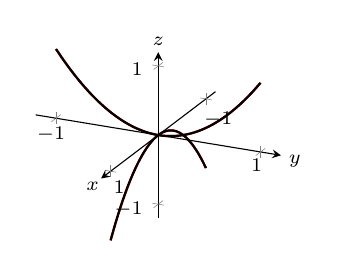
\begin{tikzpicture}[>=stealth]
\begin{axis}%
[width=175pt,tick label style={font=\scriptsize},axis on top,
			axis lines=center,
			view={115}{30},
			name=myplot,
			xtick={-1,1},
			ytick={-1,1},
			ztick={-1,1},
			ymin=-1.2,ymax=1.2,
			xmin=-1.2,xmax=1.2,
			zmin=-1.2, zmax=1.2,
			every axis x label/.style={at={(axis cs:\pgfkeysvalueof{/pgfplots/xmax},0,0)},xshift=-3pt,yshift=-3pt},
				xlabel={\scriptsize $x$},
			every axis y label/.style={at={(axis cs:0,\pgfkeysvalueof{/pgfplots/ymax},0)},xshift=5pt,yshift=-2pt},
				ylabel={\scriptsize $y$},
				every axis z label/.style={at={(axis cs:0,0,\pgfkeysvalueof{/pgfplots/zmax})},xshift=0pt,yshift=4pt},
				zlabel={\scriptsize $z$}
			]

%\addplot3[domain=-1:1,smooth,y domain=-1:1,surf,%fill=white,
%colormap={mp2}{\colormapplaneone},faceted color=black!40,samples=20,samples y=25,very thin,z buffer=sort] ({x},{y},{y^2-x^2});


\ifthenelse{\boolean{colorprint}}{%
%%%%%  Printing in color
\addplot3[domain=-1:1,,thick,smooth,samples y=0,red,%surf,%fill=white,
samples=30,] ({0},{x},{x^2});

\addplot3[domain=-1:1,,thick,smooth,samples y=0,red,%surf,%fill=white,
samples=30,] ({x},{0},{-x^2});

%%% end printing in color
}{%
%%% printing in BW
\addplot3[domain=-1:1,,thick,smooth,samples y=0,black,%surf,%fill=white,
samples=30,] ({0},{x},{x^2});

\addplot3[domain=-1:1,,thick,smooth,samples y=0,black,%surf,%fill=white,
samples=30,] ({x},{0},{-x^2});
%%%% end printing BW
}




\end{axis}



\end{tikzpicture}












